\documentclass[12pt]{article}
\usepackage[english]{babel}
\usepackage{natbib}
\usepackage{url}
\usepackage[utf8x]{inputenc}
\usepackage{amsmath}
\usepackage{graphicx}
\graphicspath{{images/}}
\usepackage{parskip}
\usepackage{fancyhdr}
\usepackage{vmargin}
\usepackage{todonotes}
\usepackage{booktabs}
\usepackage{makecell}
\usepackage{graphicx}
\usepackage{multirow}
\usepackage{color, colortbl}
\usepackage{float}
\usepackage{booktabs}
\usepackage{hyperref}
\usepackage{adjustbox}
\definecolor{Gray}{gray}{0.9}
\newcommand{\specialcell}[2][c]{%
	\begin{tabular}[#1]{@{}l@{}}#2\end{tabular}}

%left - top - right - bottom
\setmarginsrb{2 cm}{1.5 cm}{2 cm}{1.5 cm}{1 cm}{1.5 cm}{1 cm}{1.5 cm}
\usepackage[
backend=biber,
style=ieee,
]{biblatex}
\addbibresource{biblist.bib}

\title{Data Mining: Project Report}								% Title
\author{Pisciotta, Di Mauro, Murgese}								% Author


\makeatletter
\let\thetitle\@title
\let\theauthor\@author
\makeatother

\pagestyle{fancy}
\fancyhf{}
\rhead{\theauthor}
\lhead{\thetitle}
\cfoot{\thepage}

\begin{document}

%%%%%%%%%%%%%%%%%%%%%%%%%%%%%%%%%%%%%%%%%%%%%%%%%%%%%%%%%%%%%%%%%%%%%%%%%%%%%%%%%%%%%%%%%

\begin{titlepage}
	\centering
    \vspace*{0.5 cm}
    
\includegraphics[scale = 0.5]{logo.eps}\\[2.0 cm]	% University Logo

	\textsc{\Large A.A. 2020-2021}\\[0.5 cm]				% Course Code
	\rule{\linewidth}{0.2 mm} \\[0.4 cm]
	{ \huge \bfseries \thetitle}\\
	\rule{\linewidth}{0.2 mm} \\[5 cm]
	
	
	\begin{minipage}{0.5\textwidth}
		\begin{flushleft} \large
			
		\end{flushleft}
			\end{minipage}~
			\begin{minipage}{0.5\textwidth}
            
			\begin{flushright} \large
			\emph{\textbf{Group 1}} \\
			Gabriele Pisciotta \\
            Antonio Di Mauro \\
            Fabio Murgese \\
		\end{flushright}
        
	\end{minipage}\\[2 cm]
	
	

    
    
	
\end{titlepage}
%%%%%%%%%%%%%%%%%%%%%%%%%%%%%%%%%%%%%%%%%%%%%%%%%%%%%%%%%%%%%%%%%%%%%%%%%%%%%%%%%%%%%%%%%

\tableofcontents
\thispagestyle{empty}
\pagebreak

%%%%%%%%%%%%%%%%%%%%%%%%%%%%%%%%%%%%%%%%%%%%%%%%%%%%%%%%%%%%%%%%%%%%%%%%%%%%%%%%%%%%%%%%%
\setcounter{page}{1}
\section{Data Understanding}
The dataset contains informations about the puchases of products across the world. In this section we'll explore it analyzing the meaning of the values contained in it and their quality.

\subsection{Data semantics}

Our dataset is composed of 8 attributes:
\begin{enumerate}
    \item \texttt{BasketID}: the unique ID of each buying session. It's mainly a sequential number, but there are cases in which it starts with 'C'.
    \item  \texttt{BasketDate}: it's a date related to each purchase.
    \item  \texttt{Sale}: a continuous numerical attribute describing the cost of the product.
    \item  \texttt{CustomerID}: a discrete numerical attribute that describes each unique customer.
    \item  \texttt{CustomerCountry}: a categorical attribute representing the country in which the purchase has been done.
    \item  \texttt{ProdID}: a categorical attribute that is the ID of the bought product.
    \item  \texttt{ProdDescr}: a categorical attribute that describes the product or the purchase.
\end{enumerate}

Each row of our dataset represents the detail of a purchase receipt. In total, we have 471910 rows.

\subsection{Distribution of the variables and statistics}
Here we analyze in details the numerical attributes of our dataset. Even if CustomerID is a numerical attribute, it's not meaningful for us, so we'll describe only mean and variance of \texttt{Qta} and \texttt{Sale}. For both of them, we have 471910 non-null values:

\begin{itemize}
    \item \texttt{Qta}: 4.03 $\pm$ 83.76 
    \item \texttt{Sale}: 10.71 $\pm$ 231.35
\end{itemize}

Here we analyze the purchases for each dates during different periods of observation.

\begin{figure}[!h]
\minipage{0.32\textwidth}
  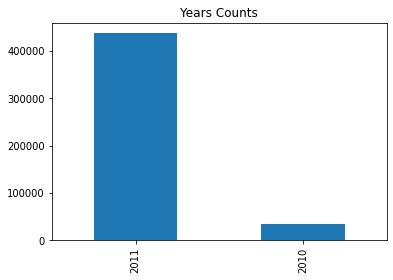
\includegraphics[width=\linewidth]{images/data1.png}
  \label{fig:data1}
\endminipage\hfill
\minipage{0.32\textwidth}
  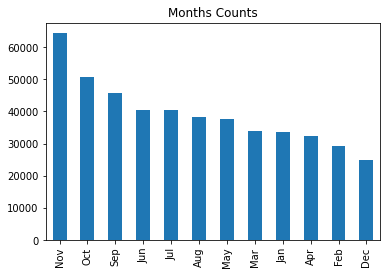
\includegraphics[width=\linewidth]{images/data2.png}
  \label{fig:data2}
\endminipage\hfill
\minipage{0.32\textwidth}%
  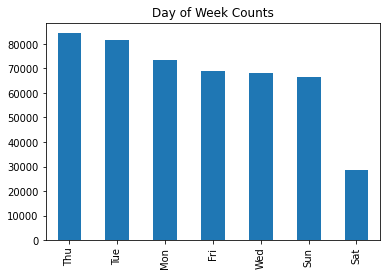
\includegraphics[width=\linewidth]{images/data3.png}
 \label{fig:data3}
\endminipage
\caption{Dates analysis}
\label{fig:triade}
\end{figure}

As we can see from Figure \ref{fig:triade}.1, we can see that almost all the purchases were done in 2011. From Figure \ref{fig:triade}.2 we can see that we have a  peak in November and the least amount in December, otherwise we can notice an almost constant behavior. From Figure \ref{fig:triade}.3 we can state that on Saturday we have half the amount of the standard.
In Figure \ref{fig:customercountry} we can observe that the vast majority of the customers are citizens of the United Kingdom, so probabily these records were taken in the UK, while recording also tourists purchases. We can see the unique values of Table \ref{table:unique_val}.

\begin{table}[h]
\centering
    \begin{tabular}{@{}llll@{}}
    \toprule
    BasketID & CustomerID & CustomerCountry & ProdID \\ \midrule
    22190 & 4372 & 37 & 3684 \\ \bottomrule
    \end{tabular}
\caption{Unique values.}
\label{table:unique_val}
\end{table}


\begin{figure}[!h]
\minipage{0.5\textwidth}
\centering
    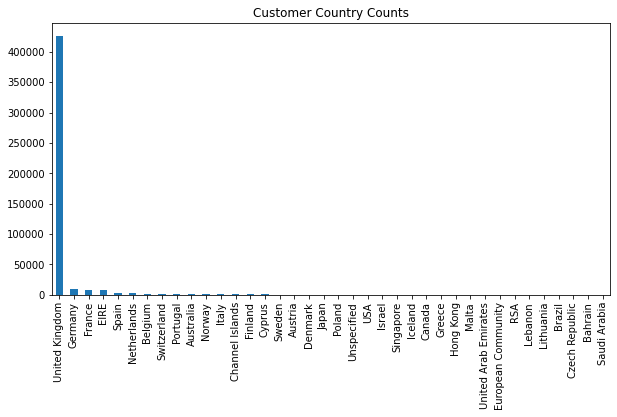
\includegraphics[scale=0.34]{customercountry.png}
    \caption{Customer country distribution.}
    \label{fig:customercountry}
\endminipage\hfill
\minipage{0.5\textwidth}
\centering
    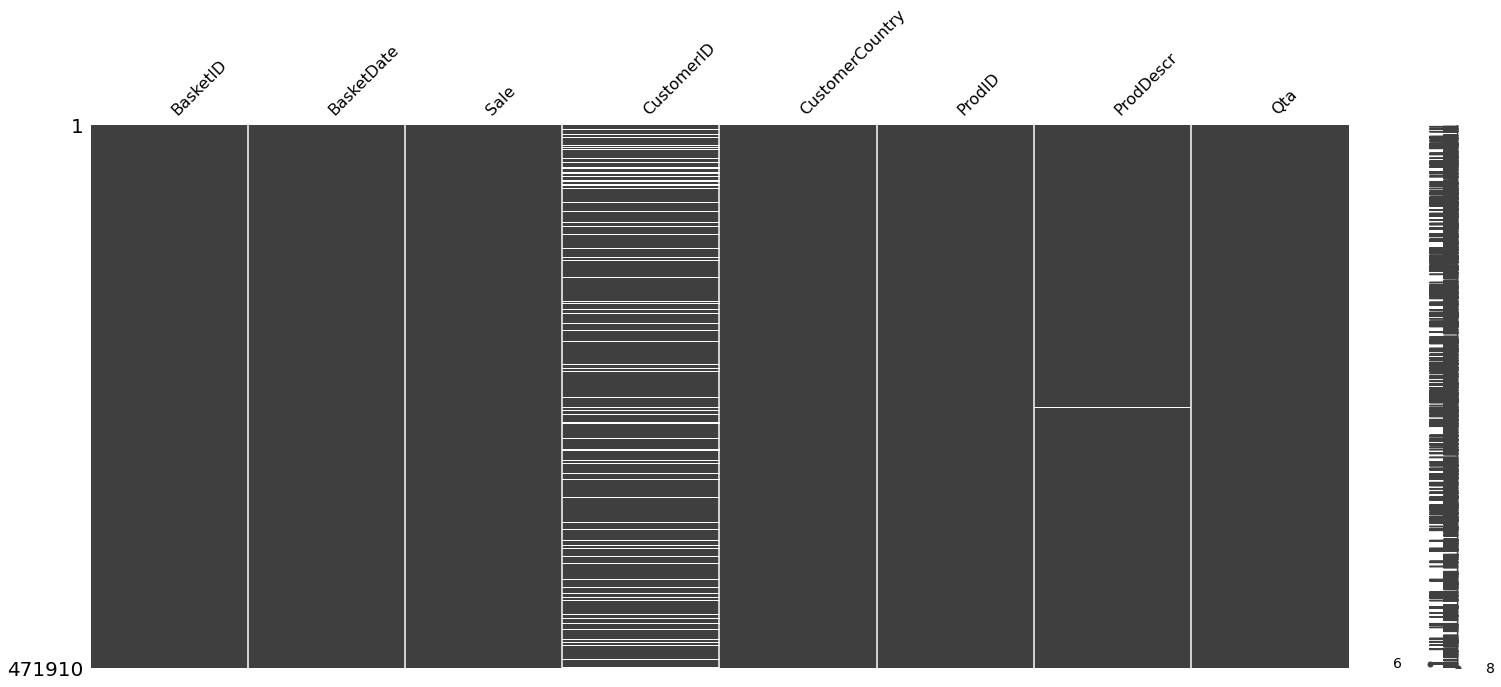
\includegraphics[scale=0.16]{images/missingValues.png}
    \caption{Missing values.}
    \label{fig:missingvalues}
\endminipage\hfill
\label{fig:customersale}
\end{figure}

We created a column \texttt{Amount} representing the total amount of money spent for each product in a basket and also analyzed this quantity with respect to the different quarters (Figure \ref{fig:boxplotq1outliers}). The Amount's values lies in 2247.01 $\pm$ 5624.24.\\
We then analyzed the total quantities bought for each product. The average quantity of sold items is 1328.05 $\pm$ 2936.95 for the entire period, despite the median is 375.50.
We can see that the mean expense for product is 3.84 $\pm$ 17.18 and that the median is 1.95. The first quartile of the products costs is 0.98 and the fourth quartile is 3.81. Also min (0.000750) and max (744.14) values have disproportionate total selling values (probably outliers).

\subsection{Assessing data quality}
Here we analyze the data quality of our dataset. By looking at Figure \ref{fig:missingvalues} it is possible to recognize the missing values of the dataset (identified by the white lines). The attribute \texttt{CustomerID} is the field with most missing values.

With the boxplot we can easily see how strange it is that very few products are so far from all the others, in terms of pricing. These are probably outliers and we'll trat them properly in the next stages.

\begin{figure}[!h]
\minipage{0.5\textwidth}
\centering
  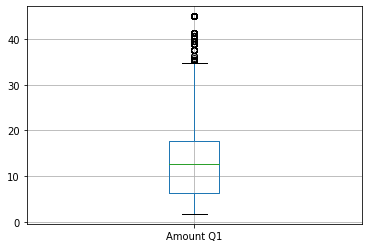
\includegraphics[scale=0.5]{images/boxplotq1outliers.png}
      \caption{Money Spent Q1 box plot.}
  \label{fig:boxplotq1outliers}
\endminipage\hfill
\minipage{0.5\textwidth}
\centering
    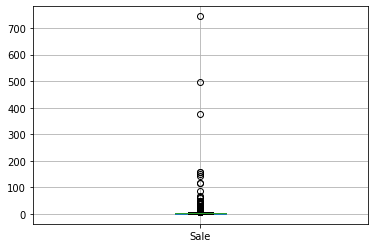
\includegraphics[scale=0.5]{images/productsboxplot.png}
    \caption{Products box plot.}
    \label{fig:productsbox}
\endminipage\hfill
\end{figure}

Let's now analyze the negative quantities in the dataset. In Table \ref{table:negative} we can see the products with negative quantities.\\ From a first view it may seem that all the \texttt{BasketID} starts with a letter 'C', but we've discovered that all the rows having negative quantities have \texttt{BasketIDs} that starts with 'C', or the vast majority of them, and also with '5'.

\begin{table}[h]
\centering
\scalebox{0.8}{

\begin{tabular}{llrrlllr}
\toprule
BasketID &          BasketDate &   Sale &  CustomerID &  ProdID &                         ProdDescr &  Qta \\
\midrule
 C536379 & 2010-01-12 09:41 &  27.50 &       14527 &       D &                          Discount &   -1 \\
 C536383 & 2010-01-12 09:49 &   4.65 &       15311 &    35004C &   SET OF 3 COLOU.... &   -1 \\
 C536391 & 2010-01-12 10:24 &   1.65 &       17548 &   22556 &  PLASTERS IN TIN....  &  -12 \\
 C536391 & 2010-01-12 10:24 &   0.29 &       17548 &    21984 &  PACK OF 12 PIN....  &  -24 \\
 C536391 & 2010-01-12 10:24 &   0.29 &       17548 &   21983 &  PACK OF 12 BLU....  &  -24 \\
\bottomrule
\end{tabular}
}
\caption{Negative values.}
\label{table:negative}
\end{table}

We noticed that \texttt{BasketIDs} that starts with '5' often don't present the \texttt{CustomerID}, while for the \texttt{BasketIDs} starting with 'C' we have only 821/9084 unspecified \texttt{CustomerIDs}. For each \texttt{BasketID} we can have multiple rows, so in order to get the right amount of \texttt{CustomerIDs} missing, we have to drop all the duplicates for each \texttt{BasketID}. After the drop, we get the proper amount of \texttt{CustomerIDs} missing: 100 / 3754. What if we remove the 'C'? Does exist any corrispondence in the main dataframe? According to the previous analysis there's no corrispondence between the \texttt{BasketIDs} having positive quantities and \texttt{BasketIDs} having negative quantities. So we can say that those are disjoint sets.\\
Also, we noticed that the description for the same \texttt{ProdID} may vary, e.g: product \textit{47566B} has 2 different descriptions that contains the reasons of that negative transaction: \textit{"reverse previous adjustment"} and \textit{"incorrectly credited C550456 see 47"}; so, we dropped some product description keeping only one. Finally we've got the main products having negative quantities with a single description, as we can see in Table \ref{tab:singledescr}.

\begin{table}[h]
    \centering
    \scalebox{0.8}{
    \begin{tabular}{llrl}
\toprule
{} &  ProdID &  Qta &                            ProdDescr \\
\midrule
0 &   23630 &    -1 &   SET 10 CARDS HANGING BAUBLES 17080 \\
1 &  85039A &    -1 &   SET/4 RED MINI ROSE CANDLE IN BOWL \\
2 &  85036A &    -1 &  GARDENIA 1 WICK MORRIS BOXED CANDLE \\
3 &   22833 &    -1 &          HALL CABINET WITH 3 DRAWERS \\
5 &   22869 &    -1 &         NUMBER TILE COTTAGE GARDEN 1 \\
\bottomrule
\end{tabular}
}
    \caption{Single description table.}
    \label{tab:singledescr}
\end{table}

From the computed statistics the majority of the negative quantities, that lies in between the first and the third quartile, are included into the interval -5/-52 but we have also negative quantities up to 80995 (almost surely an outlier).

We solved all this quality issue by removing duplicates and dropping rows having specific columns to NaN. This was enough to not having anymore inconsistencies such as BasketID with negative quantities that doesn't start with 'C'.

\section{Data Preparation}
In this section we extract new interesting features for describing the customer profile and his purchasing behavior.
We computed:
\begin{itemize}
    \item \textit{l}: the total number of items purchased by a customer during the period of observation (\texttt{Total products bought})
    \item \textit{lu}: the number of distinct items bought by a customer in the period of observation (\texttt{Distinct Products})
    \item \textit{lmax} : the maximum number of distinct products purchased by a customer during a shopping session  in the period of observation (\texttt{Max Products In Basket})
    \item \textit{E}: the \textit{Shannon entropy} of the money spent (\texttt{Entropy of money spent})
    \item the maximum, minimum and mean amount of money spent for basket
    \item the total money spent during the period of observation
    \item the maximum, minimum and mean product price in customer's basket. This value refers just to the product's value, not to the price that the customer has paid (e.g.: just the \texttt{Sale}, not \texttt{Sale} * \texttt{Qta})
    \item the quarters analysis concerning the quantities of products bought and the amount of money spent by customers.
\end{itemize}

\subsection{Variables transformations \& generation}
\begin{figure}[!h]
\minipage{0.5\textwidth}
\centering
  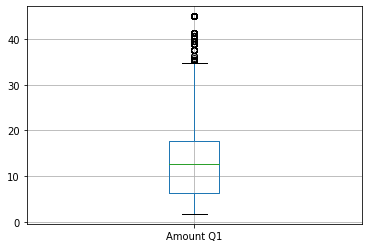
\includegraphics[scale=0.4]{images/boxplotq1outliers.png}
\endminipage\hfill
\minipage{0.5\textwidth}
\centering
  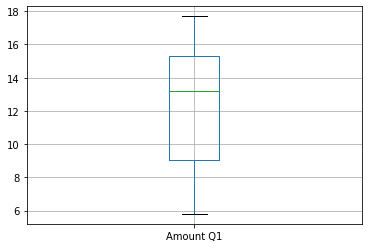
\includegraphics[scale=0.4]{images/boxplotq1.png}
\endminipage\hfill
\caption{Pre-post transformation of Amount Q1 - removal of outliers.}
\label{fig:boxplotq1outliers}
\end{figure}
We modified the original dataset identifying and eliminating the outliers (using the box plot method, e.g.:  Figure \ref{fig:boxplotq1outliers}). We also analyzed the amount of money spent on products by the customers, splitting the records by quarters of the year simulating the information needed for a business intelligence task.
\begin{figure}[!ht]
    \centering
    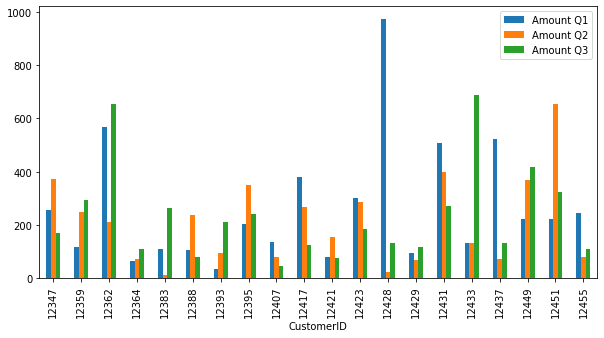
\includegraphics[scale=0.4]{images/quarters.png}
    \caption{Quarters expense for customers.}
    \label{fig:quarters}
\end{figure}
In Figure \ref{fig:quarters} we can see the comparison between just 20 customers (for the sake of presentation) representing the total quantities bought in the 3 different quarters of the year. Also, we made the same analysis for semesters and trimesters, having similar results.

\subsection{Correlation analysis}
As we can see from Figure \ref{fig:kmeans_7} the quantities and the amounts registered in the same quarter are very highly correlated, so more the products bought, more the expense. While in different quarters we notice slightly different habits in purchases by customers, still having a quite high correlation. We have groups of features that are correlated (e.g.: correlation $\ge$ 0.80), for example the quantity of products bought in a quarter and the money spent. We take this information into account for the next steps, in order to avoid to add redundant information in the clustering and the predictive analysis, that may lead to wrong deduction.


\begin{figure}[H]
\minipage{0.4\textwidth}

    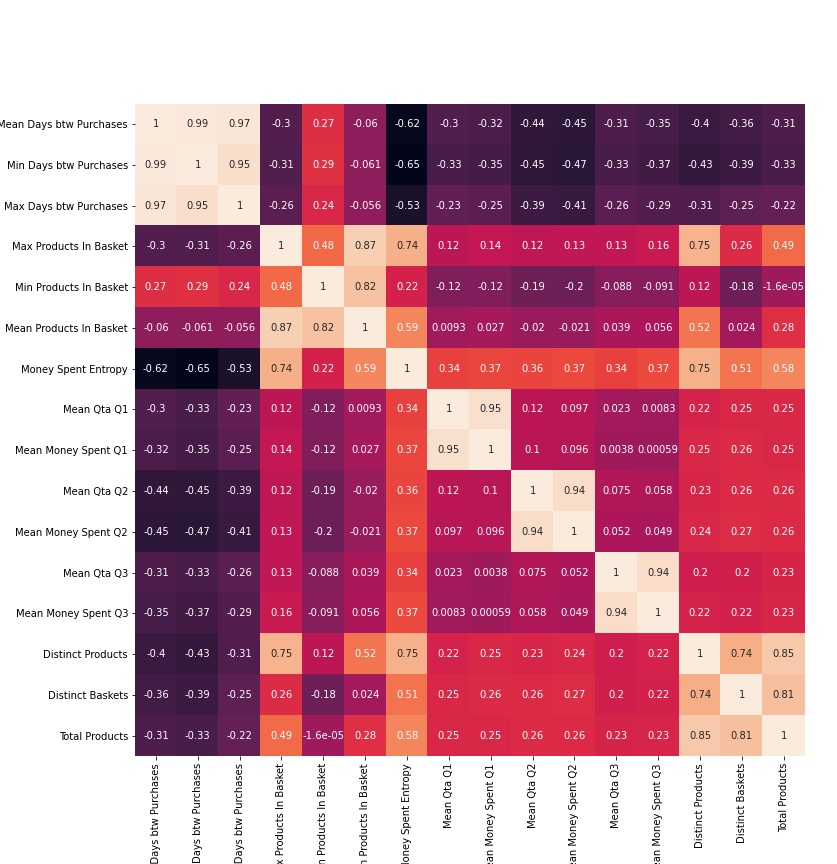
\includegraphics[scale=0.3]{images/figure_correlation_matrix_behavior(1).png}
    \caption{Correlation matrix.}
    \label{fig:kmeans_7}
    \endminipage\hfill
\minipage{0.5\textwidth}
    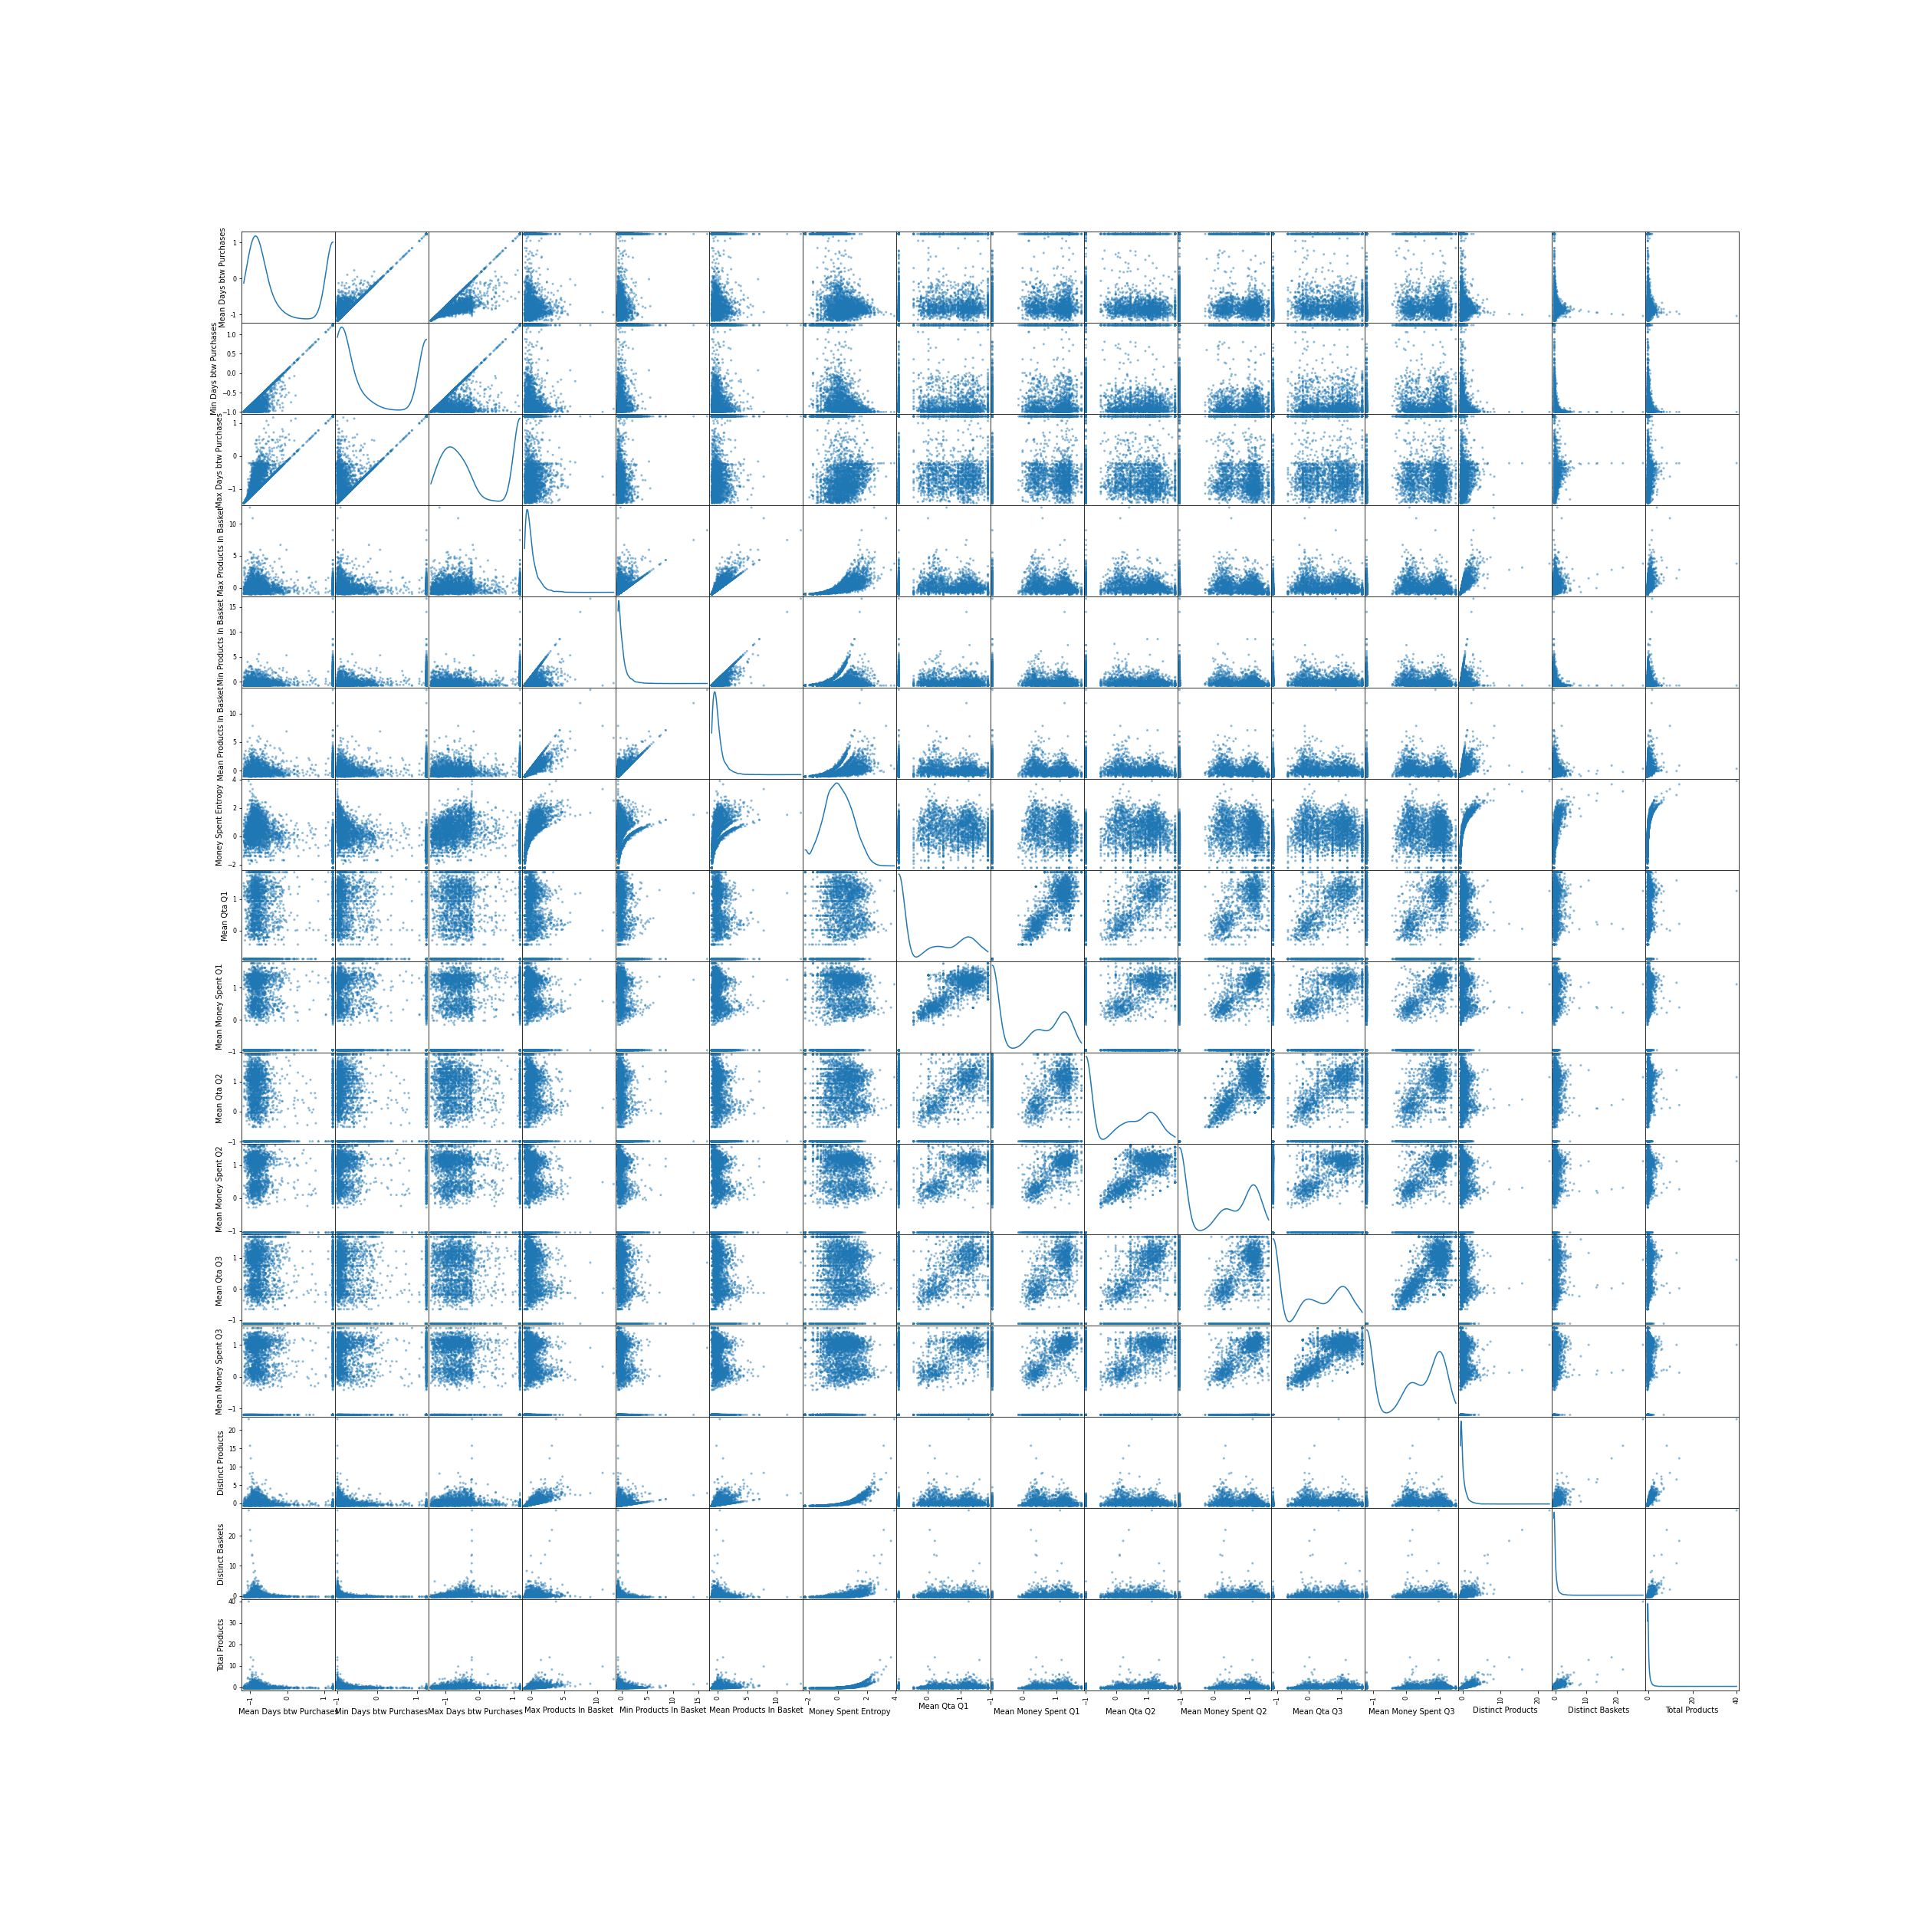
\includegraphics[scale=0.1]{images/figure_scatter_matrix_behavior.png}
    \caption{Distribution of the variables.}
     \label{fig:distribution_variables}

    \endminipage\hfill

\label{fig:insieme}
\end{figure}


\subsection{Statistics of the final dataset}
We renamed the following features with an incremental number: \texttt{Mean Days btw Purchases}, \texttt{Min Days btw Purchases}, \texttt{Max Days btw Purchases}, \texttt{Max Products In Basket}, \texttt{Min Products In Basket}, \texttt{Mean Products In Basket}, \texttt{Money Spent Entropy}, \texttt{Mean Qta Q1}, \texttt{Mean Money Spent Q1}, \texttt{Mean Qta Q2}, \texttt{Mean Money Spent Q2}, \texttt{Mean Qta Q3}, \texttt{Mean Money Spent Q3}, \texttt{Distinct Products}, \texttt{Distinct Baskets}, \texttt{Total Products}.

\begin{table}[H]
    \centering
    \tiny
\begin{tabular}{lrrrrrrrrrrrrrrrr}
\toprule
{} & 0 & 1 & 2 & 3 & 4 & 5 & 6 & 7 & 8 & 9 & 10 & 11 & 12 & 13 & 14 & 15 \\
\midrule
count &  4035 &  4035 &  4035 &  4035 &  4035 &  4035 &  4035 &  4035 &  4035 &  4035 &  4035 &  4035 &  4035 &  4035 &  4035 &   4035 \\
mean  &   340.06 &   312.02 &   380.38 &    15.58 &     7.13 &    10.84 &     2.84 &     3.92 &     6.10 &     4.11 &     6.98 &     4.81 &     7.65&    30.42&     3.75 &    295.86 \\
std   &   288.71 &   311.62&   264.58 &    14.39&     8.25 &     9.49&     1.27 &     4.35 &     6.41 &     4.14&     6.72 &     4.29 &     6.36 &    41.12&     6.27&    591.50\\
min   &     1 &     1 &     1 &     1 &     1 &     1 &     0 &     0 &     0 &     0 &     0 &     0 &     0 &     1 &     1 &      2 \\
25\%   &    87.76&    28 &   143.50 &     6 &     2 &     5 &     2.01 &     0 &     0 &     0 &     0 &     0 &     0 &     8 &     1 &     56 \\
50\%   &   167.83&   125 &   278 &    12 &     5 &     8.40 &     2.84 &     2 &     5.63&     4 &     8.11 &     4.85 &     9 &    17 &     2 &    138 \\
75\%   &   697 &   697 &   697 &    20 &     9 &    14 &     3.73&     8.33 &    13.04 &     8.06 &    14.04&     8.95 &    13.80&    39 &     4 &    342 \\
max   &   697 &   697 &   697 &   196 &   145 &   145 &     7.8 &    12 &    17.4 &    12 &    17.7 &    12 &    17.40 &   976 &   183 &  23901 \\
\bottomrule
\end{tabular}

    \caption{Variable statistics}
    \label{tab:my_label}
\end{table}

%%%%%%%%%%%%%%%%%%%%%%%%%%%%%%%%%%%%%%%%%%%%%%%%%%%%%%%%%%%%%%%%%%%%%%%%%%%%%%%%%%%%%%%%%

\section{Clustering Analysis}
In this section we analyze four different Clustering techniques applied to our data:
\begin{itemize}
    \item \textit{KMeans},
    \item \textit{DBSCAN},

    \item \textit{Hierarchical Clustering},
    \item \textit{MBSAS} (from \textsc{pyclustering} library).
\end{itemize}


\subsection{Outliers Removal with DBSCAN}
Before proceeding to the effective exploratory analysis with the different clustering techniques, we exploited \textit{DBSCAN} to detect and remove outliers from our dataset, thanks to its inherent ability to do so: it groups together points that are closely packed together (points with many nearby neighbors), marking as outliers points that lie alone in low-density regions. We chose to consider this "noisy" point as proper outliers of our dataset, and so deleting them before proceeding, and it's possible to see the difference in Figure \ref{fig:outliersremoval}.

\begin{figure}[!h]
\minipage{0.5\textwidth}
\centering
  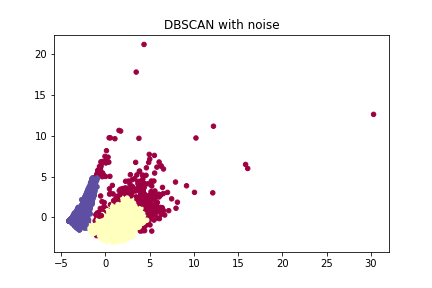
\includegraphics[scale=0.4]{images/figure_DBSCAN_outlier_removal_1.png}
\endminipage\hfill
\minipage{0.5\textwidth}
\centering
  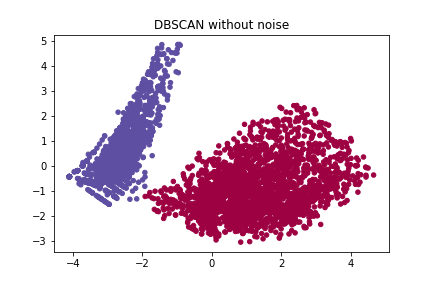
\includegraphics[scale=0.4]{images/figure_DBSCAN_outlier_removal_2.png}
\endminipage\hfill
\caption{Before and after outliers removal.}
\label{fig:outliersremoval}
\end{figure}

\subsection{KMeans}
In order to find the best clustering, we considered four types of analysis:
\begin{enumerate}
    \item on the entire dataset,
    \item on a manually selected subset of the dataset based on parallel coordinates,
    \item on a manually selected subset of the dataset,
    \item on a subset of the dataset including just the most uncorrelated features.
\end{enumerate}

For each analysis we run a grid search to find the best hyper-parameters (\textbf{numberOfClusters} $\in [2, 20]$), evaluating the results with respect to the Knee curve (\textit{SSE}). 
The best clustering is obtained with 2), taking into account a subset of the features selected using the parallel coordinates analysis generated on the entire set of features: \texttt{Distinct Products}, \texttt{Mean Days btw Purchases}, \texttt{Min Days btw Purchases}, \texttt{Max Days btw Purchases}, \texttt{Total Products}.

\begin{figure}[!h]
\minipage{0.33\textwidth}
  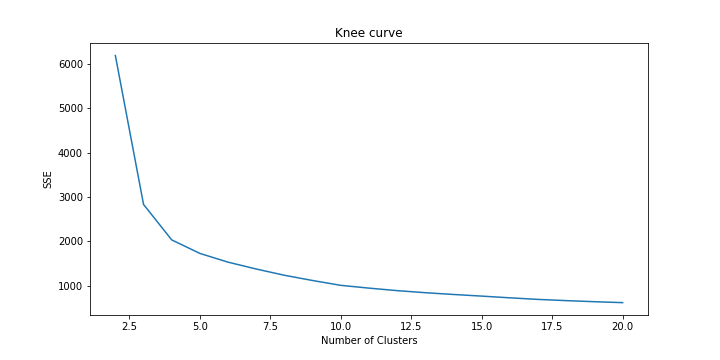
\includegraphics[scale=0.25]{images/kmeans-knee-2.png}
\endminipage\hfill
\minipage{0.33\textwidth}
  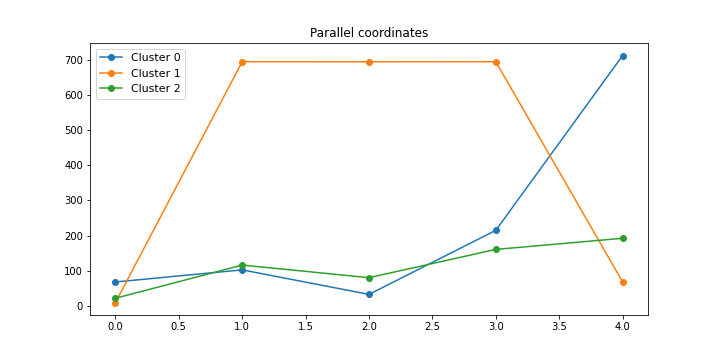
\includegraphics[scale=0.25]{images/kmeans-parcoord-2.png}
\endminipage\hfill
\minipage{0.33\textwidth}
    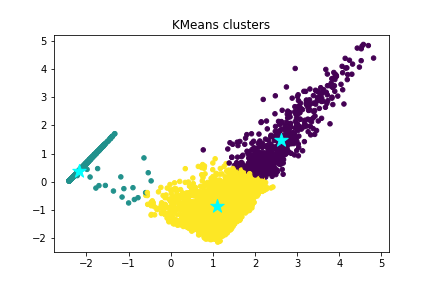
\includegraphics[scale=0.35]{images/kmeans-clusters-2.png}
    \endminipage\hfill
\caption{Knee-curve, parallel coordinates and clusters of KMeans analysis 2) }
\label{fig:kmeans_graphs}
\end{figure}

From the parallel coordinates plot in Figure \ref{fig:kmeans_graphs} we noticed that cluster 0 and 2 follow the same trend, apart from the last attribute: this means that the centroids have similar values for these attributes and so could exists some sort of correlation among this two clusters. Instead, cluster 1 follows a different characterization with respect to the other two, with features assuming different values.

\begin{table}[H]
\begin{minipage}[b]{0.5\linewidth}
\centering
    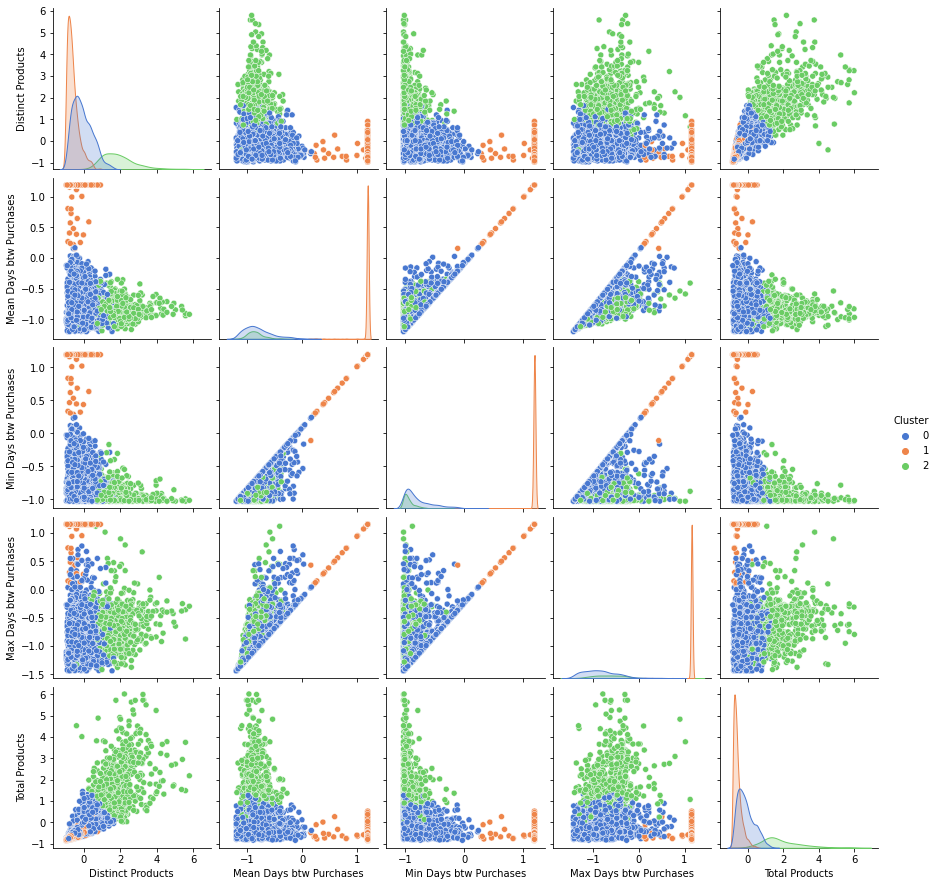
\includegraphics[scale=0.23]{images/kmeans-pairplot-2.png}
    \caption{Pairplot of features - 2).}
    \label{fig:kmeans_pairplot}
\end{minipage}
\hfill
\begin{minipage}[b]{0.5\linewidth}
\centering
\scalebox{1.1}{
    \begin{tabular}{| c | c |}
		\hline
		Number of Clusters & 3 \\
		\hline
        \rowcolor{Gray}
		Num. of init & 20 \\
		\hline
		Max iters.  & 200\\
		\hline
		\rowcolor{Gray}
		SSE score & 2833.905 \\
		\hline
		Silhouette score & 0.666\\
		\hline
		\rowcolor{Gray}
		Clusters & \specialcell{\textit{0}: 570, \\\textit{1}: 1518, \\ \textit{2}: 1636}\\
		\hline
	\end{tabular}
}
\caption{Best clustering obtained.}
\label{tab:kmeans_scores}
\end{minipage}
\end{table}

\subsubsection{Characterization}
We took into account only the feature \texttt{Mean Days btw Purchases}, instead of considering also \texttt{Min Days btw Purchases} and \texttt{Max Days btw Purchases}, because have similar distributions.\\
\textbf{Cluster 0}'s customers buy a number of distinct products that are in the mean (\texttt{Distinct Products}), they buy frequently with values around -1 (\texttt{Mean Days btw Purchases}) and they buy a lot of products on average with values around +2 (\texttt{Total Products}).\\
\textbf{Cluster 1}'s customers buy less distinct products with respect to the other clusters with values around -1 (\texttt{Distinct Products}), they buy rarely with values around +1 (\texttt{Mean Days btw Purchases}) and they buy a lot of products on average with values around +2 (\texttt{Total Products}).\\
\textbf{Cluster 2}'s customers buy more distinct products with values around +2 (\texttt{Distinct Products}), they buy rarely with values around +1 (\texttt{Mean Days btw Purchases}) and they buy less amount of total products with values around -1 (\texttt{Total Products}).

\subsection{DBSCAN}
We analyze three different approaches using DBSCAN picking the best hyper-parameters according to the Silhouette score of the clusters including the noise and without the noise:
\begin{enumerate}
    \item on the entire dataset, 
    \item on a manually selected subset of the dataset (\texttt{Mean Days between Purchases}, \texttt{Money Spent Entropy}, \texttt{Mean Products In Basket}),
    \item on a reduced dataset (PCA=2). 
\end{enumerate}

We chose to reduce the dataset to 2 dimension with the PCA because of the analysis of the variance explained in figure \ref{fig:knee_pca}. According to this analysis, with two dimension we can describe almost 80\% of the variance of the initial dataset, so we can state that it's the best trade-off between the dimensionality and the amount of information expressed in those dimensions.

\begin{table}[ht]
\begin{minipage}[b]{0.5\linewidth}
\centering
 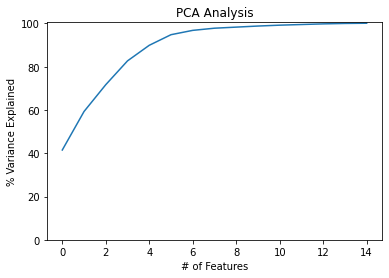
\includegraphics[scale=0.5]{images/knee_pca}
    \caption{Variance explained with PCA}
    \label{fig:knee_pca}
\end{minipage}
\hfill
\begin{minipage}[b]{0.5\linewidth}
\centering
\scalebox{1.1}{
    \begin{tabular}{| c | c |}
    \hline
	\textbf{Number of Clusters} & \textbf{2} \\
	\hline
    \rowcolor{Gray}
	Samples & 40 \\
	\hline
	Eps & 0.4\\
	\hline
	\rowcolor{Gray}
	Silhouette  & 0.475\\
	\hline
	Silhouette (w/o noise) & 0.536 \\
	\hline
    \end{tabular}
}
\caption{Best clustering obtained.}
	\label{tab:clusters_dbscan}
\end{minipage}
\end{table}

We also optimize the hyperparameters of the DBSCAN algorithm, formerly \textbf{eps} and \textbf{n\_samples}, in the following ranges:
\begin{itemize}
    \item eps: {0.1, 0.2, 0.3, 0.4, 0.5}
    \item n\_samples: {1, 2, 5, 10, 15, 20, 25, 30, 35, 40}
\end{itemize}

The resulting best approach is 2), according to the silhouette score on the clusters without noise.

\begin{figure}[!h]
\minipage{0.3\textwidth}
  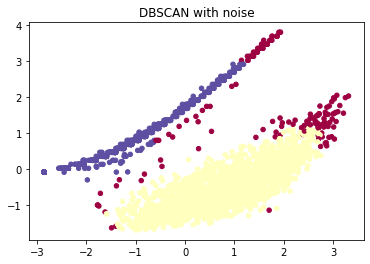
\includegraphics[scale=0.4]{images/DBSCAN_3_with.png}
\endminipage\hfill
\minipage{0.3\textwidth}
  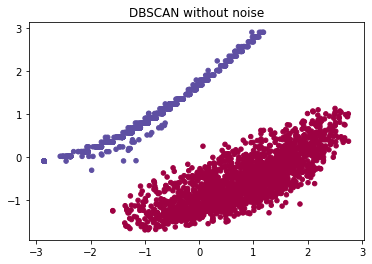
\includegraphics[scale=0.4]{images/DBSCAN_3_without.png}
\endminipage\hfill
\minipage{0.3\textwidth}
    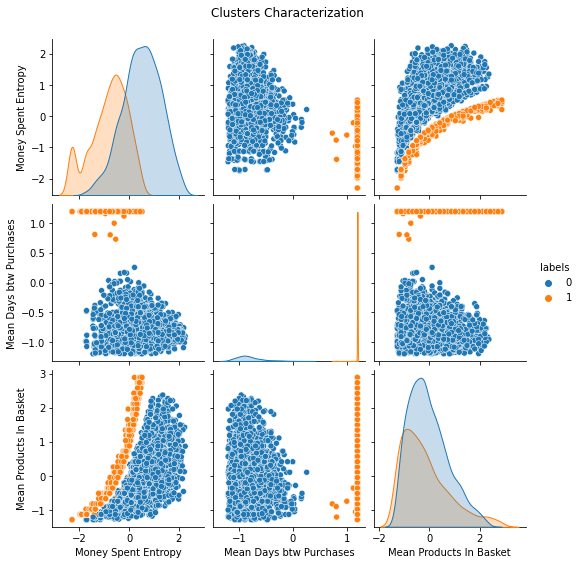
\includegraphics[scale=0.3]{images/figure_dbscan_clusters_characterization.png}
    \endminipage\hfill
\caption{Resulting clustering applying DBSCAN }
\label{fig:dbscan_3}
\end{figure}

It's possible to see that DBSCAN can cluster exploit the density of the points that in this case it's easy to interpret as two different clusters, thanks to the fact that in the previous step we already removed some outliers that lied in the middle of the space between the two blobs.

\subsubsection{Characterization}  
We compute the pairplot (Figure \ref{fig:dbscan_3}) related to that dataset, picking all the customers that aren't noise.\\ \textbf{Cluster 0}'s customers have the Money Entropy higher than the ones in Cluster 1. They also have (on average) more products in a baskets. For the frequency of buying (Mean Days between Purchases), we can note that the customers are divided between those who buy frequently (feature with value near -1) and those who buy rarely (feature with value near +1).\\ \textbf{Cluster 1}'s customers, instead, have the Money Entropy lower than the ones in Cluster 0, the frequency is very high (with values distributed around -1) and they have on average a bit less products in baskets.


\subsection{Hierarchical Clustering}
The generation of clusters with the Hierarchical approach has followed an \textbf{Agglomerative} strategy, with the usage of \textit{Euclidean} and \textit{Manhattan} distance to compute distance between points in the different clusters, and \textit{Complete}, \textit{Average}, \textit{Single} and \textit{Ward} type of linkage. We decided to operate with \textbf{numberOfClusters} $\in [2,10]$
and plotted the Silhouette score for each clustering result. The constant evidence was that after 4 or 5 clusters generated, the Silhouette scores plot dropped and the composition of the clusters was totally unbalanced, having in results one or two clusters with almost each data point in the dataset, and very few points in the remaining clusters.
We analyzed this clustering technique:
\begin{enumerate}
    \item on the entire dataset,
    \item on a manually selected subset of the dataset (\texttt{Mean Days between Purchases}, \texttt{Money Spent Entropy}, \texttt{Mean Products In Basket}),
    \item on a reduced dataset (PCA=2).
\end{enumerate}



\begin{table}[!h]
	\begin{center}
		\begin{tabular}{| c | c | c |}
			\hline
			Number of Clusters & 4 & 2 \\
			\hline
            \rowcolor{Gray}
			Linkage & \textit{Average} & \textit{Average} \\
			\hline
			Metric & \textit{Euclidean} & \textit{Manhattan}\\
			\hline
			\rowcolor{Gray}
			Silhouette score & 0.457 & 0.481 \\
			\hline
			Clusters & \specialcell{\textit{0}: 419, \\\textit{1}: 1834, \\ \textit{2}: 1090, \\ \textit{3}: 381} & \specialcell{\textit{0}: 1514, \\\textit{1}: 2210}\\
			\hline
		\end{tabular}
	\end{center}
	\caption{Clusters composition of the best clustering obtained.}
	\label{tab:clusters}
\end{table}

The best results were obtained on 2); in Table \ref{tab:clusters} we can see the composition of the best clustering obtained.

\begin{figure}[!h]
\centering
\minipage{0.4\textwidth}
  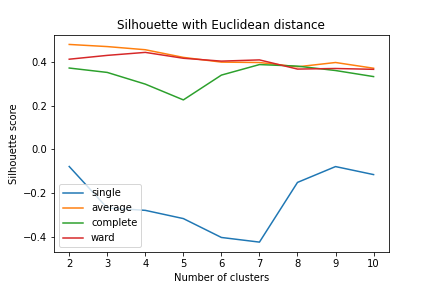
\includegraphics[width=\linewidth]{images/figure_silh_Euclidean_manually_selected_features.png}
\endminipage
\minipage{0.4\textwidth}
  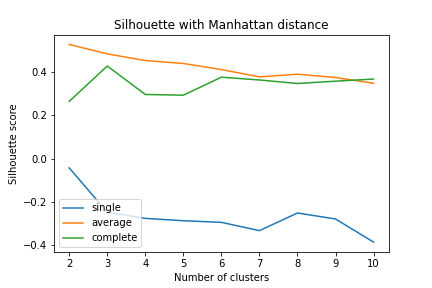
\includegraphics[width=\linewidth]{images/figure_silh_Manhattan_manually_selected_features.png}
\endminipage
\caption{Silhouette score plot.}
\label{fig:silh_hierarchical}
\end{figure}

\begin{figure}[!h]
\minipage{0.5\textwidth}
    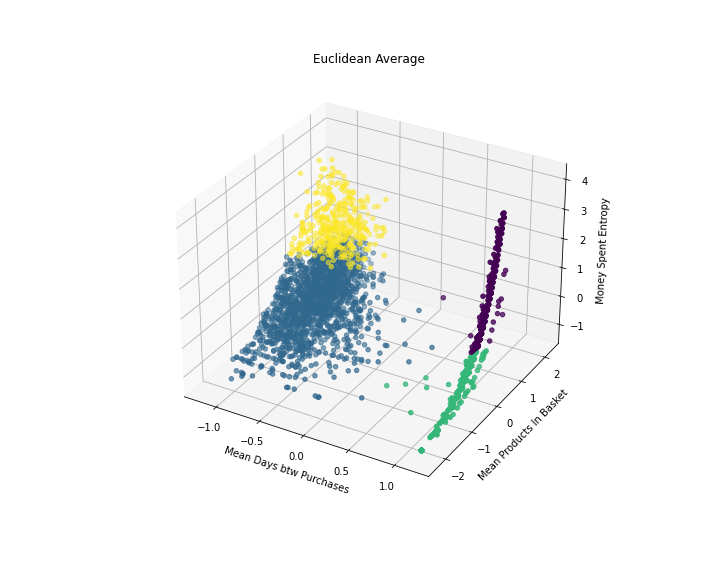
\includegraphics[width=\linewidth]{images/figure_customers_euclidean_average_selected_features_3d.png}
\endminipage\hfill
\minipage{0.5\textwidth}
  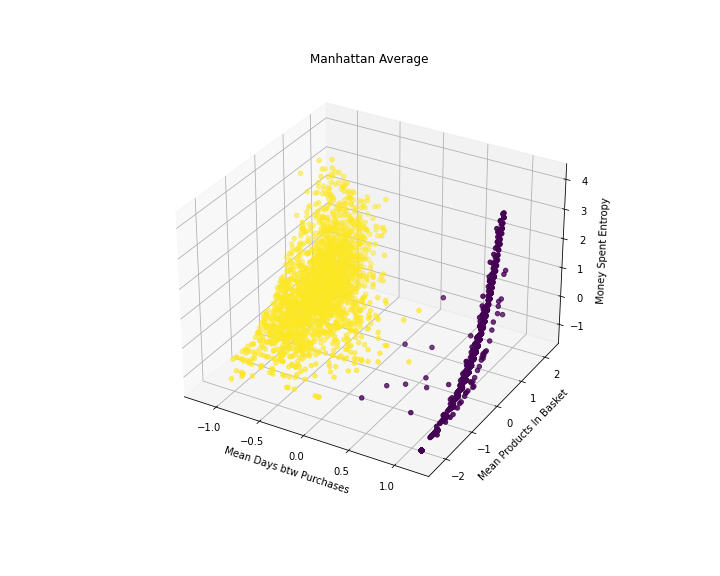
\includegraphics[width=\linewidth]{images/figure_customers_manhattan_average_selected_features_3d.png}
\endminipage\hfill
\caption{Customers visualization.}
\label{fig:customers_3d}
\end{figure}

\begin{figure}[!h]
\centering
\minipage{0.4\textwidth}
    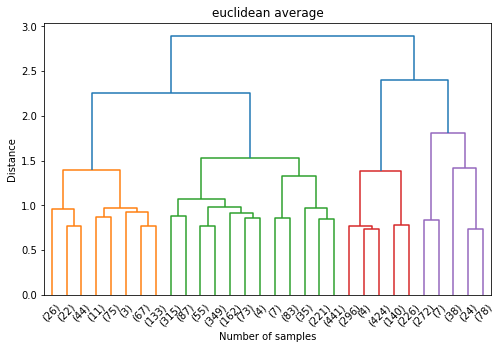
\includegraphics[width=\linewidth]{images/figure_dendr_eucl.png}
\endminipage\hfill
\minipage{0.4\textwidth}
  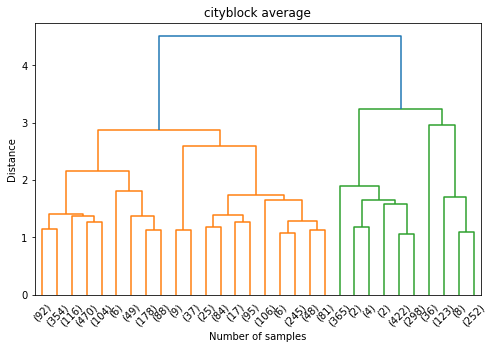
\includegraphics[width=\linewidth]{images/figure_dendr_manh.png}
\endminipage\hfill
\caption{Dendrograms of the best clustering obtained.}
\label{fig:dendrograms}
\end{figure}

\begin{figure}[!h]
\minipage{0.5\textwidth}
    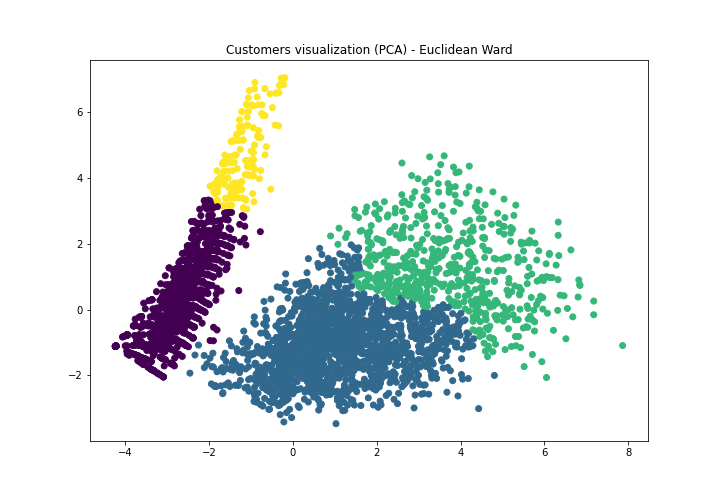
\includegraphics[width=\linewidth]{images/figure_customers_Euclidean_Ward_pca.png}
\endminipage\hfill
\minipage{0.5\textwidth}
  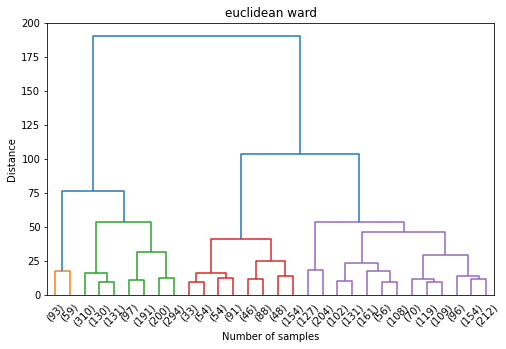
\includegraphics[width=\linewidth]{images/figure_dendr_pca.png}
\endminipage\hfill
\caption{Hierarchical clustering on \textit{PCA} reduced dataset.}
\label{fig:hierarch_pca}
\end{figure}

In Figure \ref{fig:dendrograms} we can notice how clusters are formed using different inter-cluster distances with \textit{dendrograms}, tree-like representations of the arrangement of the clusters produced. We can notice that with Euclidean Average we have points with lower distance and 4 clusters pretty much well defined. With Manhattan Average, instead, we have higher distance between data points and 2 clusters better discriminated (lower distance between higher linkages). With Single linkage, instead, we had the worst results, so we decided not to show these dendrograms.\\
Furthermore, in Figure \ref{fig:hierarch_pca} we can see the results of hierarchical clustering on the dataset reduced with \textit{PCA} (2 dimensions).

\subsection{MBSAS (optional)}
To use this clustering algorithm, we exploited the \textsc{pyclustering} library. 
The hyperparameters we tune are the \textbf{threshold} and \textbf{n\_clusters}, according to the following grid search:
\begin{itemize}
    \item threshold: [0.1, ..., 1.5, 2.0, 3.0, 5.0, 10.0, 20, 50, 100]
    \item n\_clusters: {2, 3}
\end{itemize}
The threshold specified here is the threshold of euclidean distance between the points.
We run three kind of experiment, picking the best hyperparamethers according to the silhouette
\begin{enumerate}
    \item on the entire dataset,
    \item on a manually selected subset of the dataset,
    \item on a reduced dataset (PCA=2).
\end{enumerate}

The resulting best approach is 3), according to the silhouette score that is possible to see in Table \ref{tab:clusters_mbsas}.

\begin{table}[ht]
\centering
\begin{minipage}[b]{0.4\linewidth}
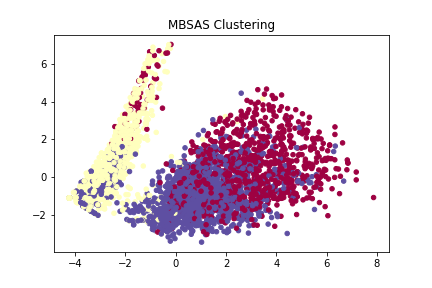
\includegraphics[width=\linewidth]{images/figure_MBSAS.png}
\caption{Results applying \textit{MBSAS}.}
\label{fig:mbsas_visualization}
\end{minipage}
\begin{minipage}[b]{0.4\linewidth}
\scalebox{1.1}{
    \begin{tabular}{| c | c |}
    	\hline
    	\textbf{Number of Clusters} & \textbf{3} \\
    	\hline
        \rowcolor{Gray}
    	Threshold & 5.0 \\
    	\hline
    	Eps & 0.4\\
    	\hline
    	\rowcolor{Gray}
    	Silhouette  & 0.396\\
    	\hline
    \end{tabular}
}
\caption{MBSAS clusters composition}
\label{tab:clusters_mbsas}
\end{minipage}
\end{table}

It's possible to see from \ref{fig:mbsas_visualization} that the clusters that emerges are somehow 'noisy', this is due to the nature of the \textit{MBSAS} algorithm which is highly influenced by the order of presentation of the data points and the distance from the representative according to the whole sequence, considering also a distance threshold. It's possible to see from the notebook that the result may vary a lot changing the hyperparameters of the clustering algorithm (upper bound of the number of clusters and distance threshold). 

\subsection{Best Clustering results}
We can see that the best results obtained with a clustering techniques are obtained with KMeans. It's the method that presents the best results according to the silhouette as we can see in Table \ref{tab:kmeans_scores}. For what concerns DBSCAN, it is very good at identifying cluster based on their density, and in the Figure \ref{fig:dbscan_3} emerges quickly its ability to consider the two manifolds. We noticed, from the results in Table \ref{tab:clusters} that also the Hierachical achieves a good silhouette score. In general, the advantage of agglomerative hierarchical clustering is that it tends to produce more accurate results. The downside is that hierarchical clustering is more time/resource consuming than the others. We in the end consider DBSCAN a really good approach because it have an high silhouette score and its also useful because of its ability to detect noisy points and let us remove them, instead of trying to assign them to clusters.

%%%%%%%%%%%%%%%%%%%%%%%%%%%%%%%%%%%%%%%%%%%%%%%%%%%%%%%%%%%%%%%%%%%%%%%%%%%%%%%%%%%%%%%%%%%%
\section{Predictive Analysis}
In this section we analyze different classification models we used in order to predict the customer's spending behavior:
\begin{itemize}
    \item \textit{K-Nearest Neighbors}
    \item \textit{Support Vector Machine} for Classification
    \item \textit{Decision Tree}
    \item \textit{Random Forest}
    \item \textit{MultiLayer Perceptron}
\end{itemize}
In Table \ref{tab:hyper} we can see the algorithms used and the hyper-parameters tried for the experiments.
The hyperparameter search has been done with a 5-Fold Grid Search cross validation strategy(2-Fold for MLP), selecting the best according to the mean F1 validation score.

\begin{table}[h]
		        \begin{center}

		\scalebox{0.5}{
    
		\begin{tabular}{| c | l |}
		
			\hline
			\textbf{Algorithm} & \textbf{Hyper-parameters}\\
			\hline
			
            \rowcolor{Gray}
			KNN & \specialcell{
				\textit{n\_neighbors} : 5, 20, 50 \\
				\textit{weights} : 'uniform', 'distance' \\
				\textit{algorithm}: 'ball\_tree', 'kd\_tree', 'brute'} \\
			\hline
			
			SVC & \specialcell{
			\textit{C}: 1, 0.5, 0.1, 0.01, 0.001 \\
			\textit{gamma}: 'auto'\\
			\textit{kernel}: 'linear', 'rbf' \\
			\textit{class\_weight}: 'balanced', None }\\
			\hline
			
			\rowcolor{Gray}
			Decision Tree & \specialcell{
				\textit{criterion} : 'gini'\\
				\textit{max\_depth} : None\\
				\textit{min\_samples\_split} : 2}\\
			\hline
			
			Random Forest & \specialcell{
			    \textit{max\_depth} : 10, 20, 50, None \\
			    \textit{max\_features}: 'auto' \\
			    \textit{min\_samples\_split} : 2, 5, 10 \\
			    \textit{min\_samples\_leaf} : 1, 2, 4 \\
			    \textit{bootstrap} : True, False \\
			    \textit{n\_estimators}: 100, 200 \\
			    \textit{criterion} : 'entropy', 'gini' \\
			    \textit{class\_weight} : 'balanced', None}\\
			\hline
			
			\rowcolor{Gray}
			MultiLayer Perceptron & \specialcell{
			    \textit{lr} : 0.0001, 0.0002, 0.0003, 0.01, 0.02, 0.03, 0.1, 0.2, 0.3 \\
			    \textit{lr\_decay} : 0.9, 0.8 \\
			    \textit{decay\_steps} : 10000, 100000 \\
			    \textit{epochs} : 200, 300, 500, 750, 1000 \\
			    \textit{batch\_size} : 5, 10, 25, 50 \\
			    \textit{lambda} : 1e-5, 1e-6, 1e-7 \\
			    \textit{hidden\_layers} : 2 \\}\\
			\hline
		\end{tabular}
	}
			\end{center}

	\caption{Setup environment of the tested hyper-parameters.}
	\label{tab:hyper}
\end{table}

\subsection{Label Generation}
First of all, we needed to assign different labels to our customers: \textbf{high spending, medium spending, low spending}.
These labels have been assigned based on a combination of selected features that allowed us to give each record (customer) the proper label. We decided to follow a \textit{Supervised Discretization} approach based on the percentiles of the following features: 
\begin{itemize}
    \item \texttt{Money Spent Entropy}
    \item \texttt{Mean Days between Purchases}
    \item \texttt{Mean Products In Basket}
    \item \texttt{Mean Qta} (sum of the mean quantity for each quarter of the year)
    \item \texttt{Mean Money Spent} (idem)
\end{itemize}
This let us have robust features according to the time of observation and also according to generalization purposes, in order to classify correctly also relatively new users. \begin{table}[]

    \centering
    		\scalebox{0.7}{

    \begin{tabular}{l c}
    \toprule
    {Customer type} &  \# of examples \\
    \midrule
    high-spending   &            772 \\
    low-spending    &            681 \\
    medium-spending &           2271 \\
    \bottomrule
    \end{tabular}
    }
    \caption{Distribution of examples for each label.}
    \label{table:number_of_examples}

\end{table}
We can see from Table \ref{table:number_of_examples} that we have a sort of Gaussian distribution about the number of examples centered in the medium-spending category. This is reasonable due to the fact that we can assume that this phenomena, with increasing number of customers, we'll have more and more medium-spending ones, while high-spending and low-spending will increase at a slower rate. We can suppose that a good enough explanation for this is the law of large numbers.



\subsection{K-Nearest Neighbors}
At the end of the cross validation, we picked the best hyper-parameters:
\begin{table}[h]
\centering
\begin{tabular}{lcccc}
\toprule
 preprocessing & n\_neighbors & weights & algorithm &  mean\_valid\_f1 \\
\midrule
No scaler &             5 & distance &              ball\_tree &            0.896 \\
Standard scaler                  &                        5 &             distance &              ball\_tree &            0.919 \\
\bottomrule
\end{tabular}
\end{table}

We used these parameters to re-train the classifier on the whole training set and then computed the metrics for both training set and test set. 

%%%%%%%%%%%%%%%%%%%%%%%%%%%%%%%%%%%
\begin{table}[ht]
\begin{minipage}[b]{0.5\linewidth}
\centering
    \vfill
    \begin{tabular}{@{}lccc@{}}
    \toprule
     & \multicolumn{1}{l}{F1} & \multicolumn{1}{l}{P} & \multicolumn{1}{l}{R } \\ \midrule
    Train & 1.0  & 1.0 & 1.0 \\
    Test & 0.915 & 0.915 & 0.897 \\ \bottomrule
    \end{tabular}
    \vfill

\caption{Metrics (macro)}
\label{table:knn_res}
\end{minipage}\hfill
\begin{minipage}[b]{0.5\linewidth}
\centering
    \vfill
    \begin{tabular}{@{}lccc@{}}
    \toprule
     & \multicolumn{1}{l}{F1} & \multicolumn{1}{l}{P} & \multicolumn{1}{l}{R } \\ \midrule
    Train & 1.0  & 1.0 & 1.0 \\
    Test & 0.929 & 0.945 & 0.916 \\ \bottomrule
    \end{tabular}
    \vfill
\caption{Metrics (macro) (standardized)}
\label{table:knn_res}
\end{minipage}\hfill
\end{table}

\begin{table}[ht]
\begin{minipage}[b]{0.5\linewidth}
\centering
    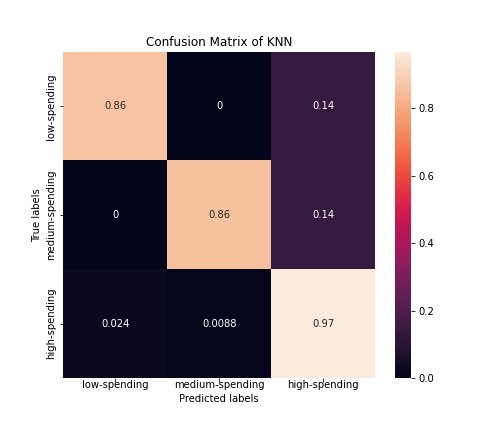
\includegraphics[scale=0.5]{images/figure_KNN_without_scaler.png}
\caption{Confusion Matrix}
\label{fig:image}
\end{minipage}
\begin{minipage}[b]{0.5\linewidth}
\centering
    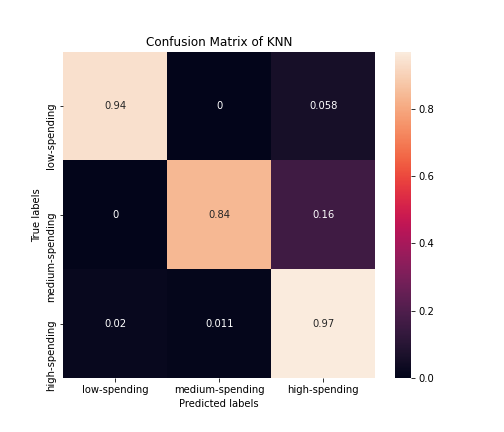
\includegraphics[scale=0.5]{images/figure_KNN_with_scaler.png}
\caption{Confusion Matrix (standardized)}
\label{fig:image}
\end{minipage}
\end{table}
%%%%%%%%%%%%%%%%%%%%%%%%%%%%%%%%%%%%%%%%%%%%%%%%%%%%%%%%%%%%%%%%%%%%5

\newpage
\subsection{SVM}
At the end of the cross validation, we picked the best hyper-parameters:
\begin{table}[h]
\centering
\begin{tabular}{lccccc}
\toprule
 preprocessing & C & class\_weights & gamma &  kernel & mean\_valid\_f1 \\
\midrule
No scaler                  &           0.01 &                  balanced &               auto &              linear &             0.859 \\
Standard scaler                 &              1 &                      None &               auto &                 rbf &            0.920 \\
\bottomrule
\end{tabular}
\end{table}

We used these parameters to re-train the classifier on the whole training set and then computed the metrics for both training set and test set. 

%%%%%%%%%%%%%%%%%%%%%%%%%%%%%%%%%%%
\begin{table}[ht]
\begin{minipage}[b]{0.5\linewidth}
\centering
    \vfill
    \begin{tabular}{@{}lccc@{}}
    \toprule
     & \multicolumn{1}{l}{F1} & \multicolumn{1}{l}{P} & \multicolumn{1}{l}{R } \\ \midrule
    Train & 0.860 & 0.834 & 0.914 \\
    Test & 0.839 & 0.815 & 0.893 \\ \bottomrule
    \end{tabular}
    \vfill

\caption{Metrics (macro)}
\label{table:knn_res}
\end{minipage}\hfill
\begin{minipage}[b]{0.5\linewidth}
\centering
    \vfill
    \begin{tabular}{@{}lccc@{}}
    \toprule
     & \multicolumn{1}{l}{F1} & \multicolumn{1}{l}{P} & \multicolumn{1}{l}{R } \\ \midrule
    Train & 0.93 & 0.955 & 0.909 \\
    Test & 0.916 & 0.949 & 0.892 \\ \bottomrule
    \end{tabular}
    \vfill
\caption{Metrics (macro) (standardized)}
\label{table:knn_res}
\end{minipage}\hfill
\end{table}

\begin{table}[ht]
\begin{minipage}[b]{0.5\linewidth}
\centering
    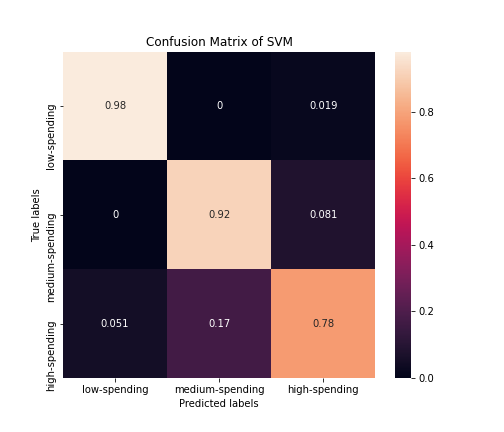
\includegraphics[scale=0.5]{images/figure_SVM_without_scaler.png}
\caption{Confusion Matrix}
\label{fig:image}
\end{minipage}
\begin{minipage}[b]{0.5\linewidth}
\centering
    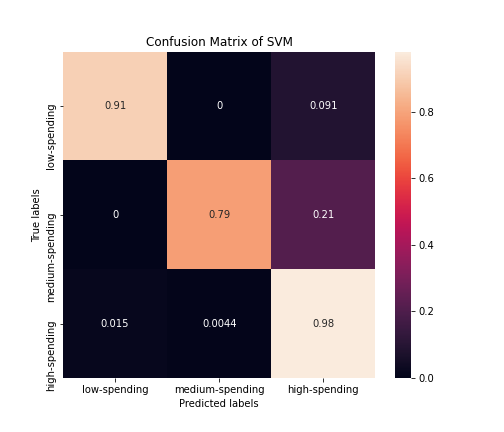
\includegraphics[scale=0.5]{images/figure_SVM_with_scaler.png}
\caption{Confusion Matrix (standardized)}
\label{fig:image}
\end{minipage}
\end{table}
%%%%%%%%%%%%%%%%%%%%%%%%%%%%%%%%%%%%%%%%%%%%%%%%%%%%%%%%%%%%%%%%%%%%5

\newpage
\subsection{Decision Tree}
For the Decision Tree we leaved the hyper-parameters listed in Table \ref{tab:hyper}. We run it on the non standardized dataset, obtaining the following results:

\begin{table}[h]
    \centering
    \begin{tabular}{@{}lccc@{}}
    \toprule
     & \multicolumn{1}{l}{F1} & \multicolumn{1}{l}{P} & \multicolumn{1}{l}{R } \\ \midrule
    Train & 1.0 & 1.0 & 1.0 \\
    Test & 1.0 & 1.0 & 1.0 \\ \bottomrule
    \end{tabular}
    \caption{Metrics (macro)}
    \label{tab:metrics_decision_tree}
\end{table}
Considering the perfect results, we avoided to insert in this report the confusion matrix with its obvious content.
A more interpretable way to look at the Decision Tree results is with the Figure \ref{fig:decision_tree_explained}:
\begin{figure}[h]
    \centering
    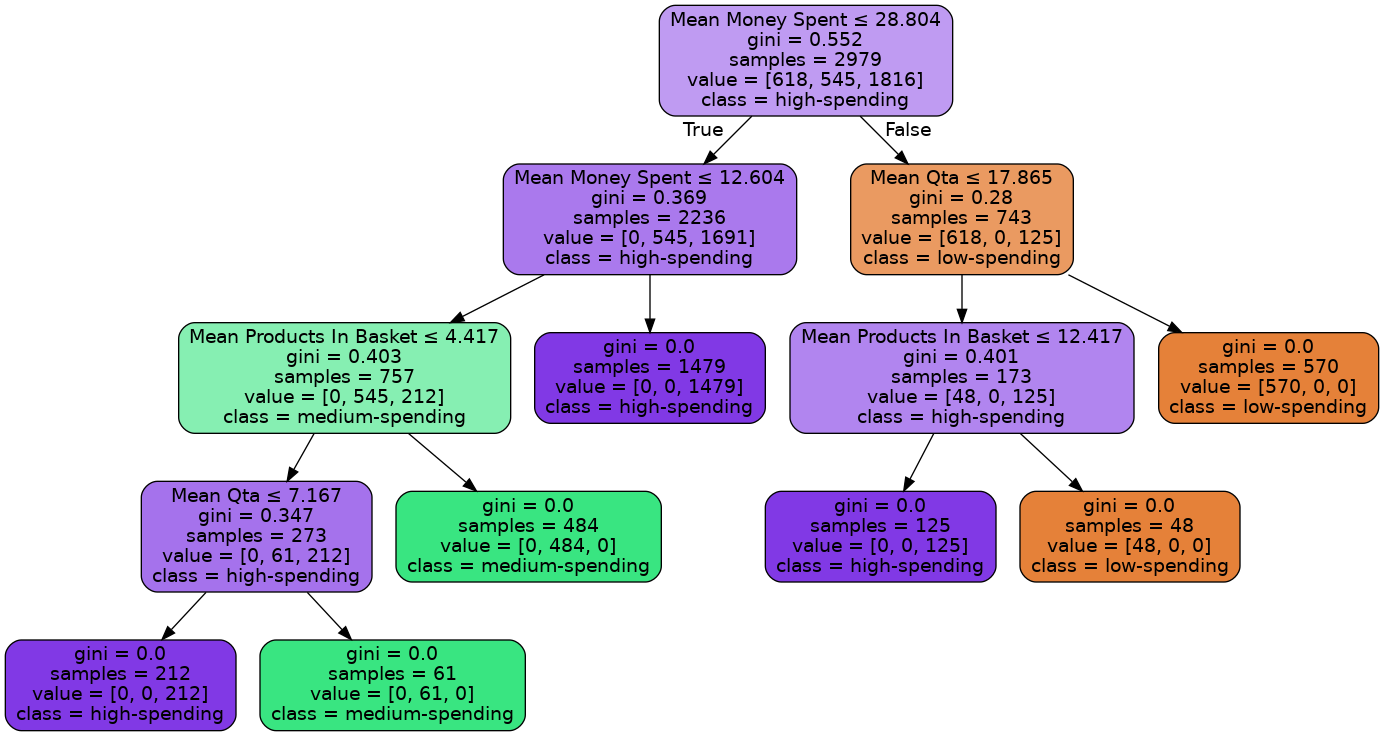
\includegraphics[scale=0.35]{images/figure_decision_tree.png}
    \caption{Decision Tree explained}
    \label{fig:decision_tree_explained}
\end{figure}

\newpage
\subsection{Random Forest}
For the Random Forest we picked the best hyper-parameters listed in Table \ref{tab:random_forest_best_hyper}. We run it on the non standardized dataset, obtaining the results listed in Table \ref{tab:metrics_random_forest}.

\begin{table}[H]
\centering
\begin{tabular}{cccccc}
\toprule
 max\_depth & min\_samples\_split & min\_samples\_leaf & bootstrap & n\_estimators & criterion \\
\midrule
10 & 2 & 2 & False & 200 & 'gini' \\
\bottomrule
\end{tabular}
\caption{Random Forest best hyper-parameters}
\label{tab:random_forest_best_hyper}
\end{table}

\begin{table}[h]
    \centering
    \begin{tabular}{@{}lccc@{}}
    \toprule
     & \multicolumn{1}{l}{F1} & \multicolumn{1}{l}{P} & \multicolumn{1}{l}{R } \\ \midrule
    Train & 1.0 & 1.0 & 1.0 \\
    Test & 1.0 & 1.0 & 1.0 \\ \bottomrule
    \end{tabular}
    \caption{Metrics (macro)}
    \label{tab:metrics_random_forest}
\end{table}

\begin{figure}[h]
    \centering
    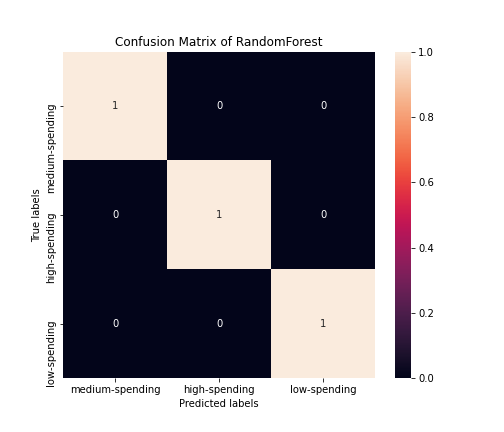
\includegraphics[scale=0.55]{images/figure_RandomForest.png}
    \caption{Random Forest confusion matrix}
    \label{fig:random_forest}
\end{figure}

\newpage
\subsection{MultiLayer Perceptron}
After the model selection phase, we picked the best hyper-parameters:
\begin{table}[H]
\centering
\begin{tabular}{lccccccc}
\toprule
 lr & lr\_decay & epochs & batch\_size & lambda & n\_hidden & decay\_steps & optimizer \\
\midrule
0.0001 & 0.9 & 1000 & 25 & 1e-7 & 15 & 10000 & 'Adam' \\
\bottomrule
\end{tabular}
\caption{MLP best hyper-parameters for both the experiments}
\label{tab:mlp_best_hyper}
\end{table}

After the model assessment phase using the parameters in Table \ref{tab:mlp_best_hyper}, we executed the predictions of the model on the  test set. The results obtained are shown in the following tables:


%%%%%%%%%%%%%%%%%%%%%%%%%%%%%%%%%%%
\begin{table}[ht]
\begin{minipage}[b]{0.5\linewidth}
\centering
    \vfill
    \begin{tabular}{@{}lccc@{}}
    \toprule
     & \multicolumn{1}{l}{F1} & \multicolumn{1}{l}{P} & \multicolumn{1}{l}{R } \\ \midrule
    Train & 0.909 & 0.929 & 0.892 \\
    Test & 0.913 & 0.933 & 0.897 \\ \bottomrule
    \end{tabular}
    \vfill

\caption{Metrics (macro)}
\label{table:mlp_res}
\end{minipage}\hfill
\begin{minipage}[b]{0.5\linewidth}
\centering
    \vfill
    \begin{tabular}{@{}lccc@{}}
    \toprule
     & \multicolumn{1}{l}{F1} & \multicolumn{1}{l}{P} & \multicolumn{1}{l}{R } \\ \midrule
    Train & 0.940 & 0.968 & 0.961 \\
    Test & 0.967 & 0.967 & 0.967 \\ \bottomrule
    \end{tabular}
    \vfill
\caption{Metrics (macro) (standardized)}
\label{table:mlp_res_2}
\end{minipage}\hfill
\end{table}

\begin{table}[ht]
\begin{minipage}[b]{0.5\linewidth}
\centering
    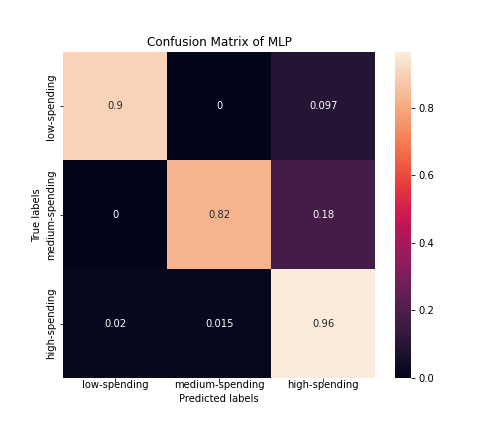
\includegraphics[scale=0.5]{images/mlp-confusionmatrix_without_std.png}
\caption{Confusion Matrix}
\label{fig:mlp_conf}
\end{minipage}
\begin{minipage}[b]{0.5\linewidth}
\centering
    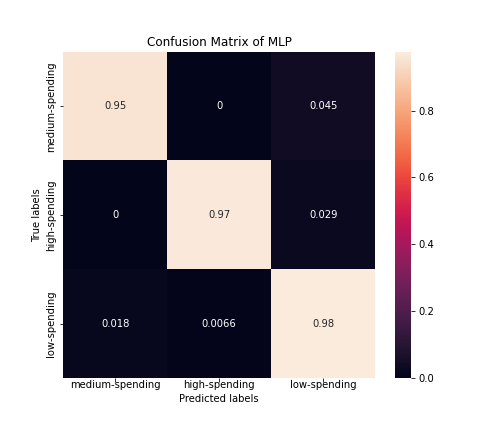
\includegraphics[scale=0.5]{images/mlp-confusionmatrix.png}
\caption{Confusion Matrix (standardized)}
\label{fig:mlp_conf2}
\end{minipage}
\end{table}
%%%%%%%%%%%%%%%%%%%%%%%%%%%%%%%%%%%%%%%%%%%%%%%%%%%%%%%%%%%%%%%%%%%%5


\subsection{Best Classification model}

Guided by the metrics computed on the test set for estimating the generalization error and by the "Occam’s Razor rule", we consider as the best classification model the Decision Tree, because of its simplicity and its perfect score. We can observe in Figure \ref{fig:decision_tree_explained} how it can reproduce in a perfect way the label generation method we used, exploiting the quartiles of the features involved. Also the Random Forest, being an ensemble of Decision Tree, achieves perfect results, but being more complex in terms of architecture, being an ensemble of Decision Tree. We chose the simple Decision Tree also for its explainability by default, without involving external tools.
For the other models experimented, we noted that there are some misclassified examples, probably due to class imbalance. We exploited also the standardization as preprocessing, which let us achieve better results when involved. As future works to improve the classification, we could consider methods of oversampling / undersampling to try to re-balance the dataset, but the label generation rule up to now is quite simple and the use of a Decision Tree model fit perfectly. For more complex rules and definition of "spendent", more complex classifiers (and also set of features) should be tested: for example, from the results in table \ref{table:mlp_res_2} we can see that the MLP model is quite flexible and is the second best model.

\section{Sequential Pattern Mining}
\subsection{Generalized Sequential Pattern}
To use this algorithm, we exploited the \textsc{SPMF}\footnote{\url{http://www.philippe-fournier-viger.com/spmf/}} library, thanks to the opportunity to also use it for timing constraints. We experimented also the suggested \texttt{gsp.py} script, but we noticed that for our dataset it was very slow (order of hours), while with the Java implementation we're able to complete the analysis in few minutes.\\
We run experiments with different value of support: 3.5\%, 5\% and 10\%, noting that the higher the support, the less the sequences obtained.
With 5\% support we got \texttt{177} sequences and we reported some of them in Table \ref{tab:rules_no_constr_5}.

\begin{table}[H]
\centering
\scalebox{0.7}{

\begin{tabular}{l c}
\toprule
 Sequence & Support \\
\midrule
    CREAM HANGING HEART T-LIGHT HOLDER, CREAM HANGING HEART T-LIGHT HOLDE & 416 \\
    REGENCY CAKESTAND 3 TIER, REGENCY CAKESTAND 3 TIER & 363 \\
    \centerline{\vdots} \\
    LUNCH BAG RED RETROSPOT, LUNCH BAG SPACEBOY DESIGN & 201 \\
    LUNCH BAG RED RETROSPOT, JUMBO BAG RED RETROSPOT & 201 \\
    \centerline{\vdots} \\
    PARTY BUNTING, CREAM HANGING HEART T-LIGHT HOLDER & 169 \\
    LUNCH BAG SUKI DESIGN, LUNCH BAG PINK POLKADOT & 169 \\
    LUNCH BAG CARS BLUE, LUNCH BAG ALPHABET DESIGN & 169 \\
\bottomrule
\end{tabular}
}
\caption{Sequences ordered by support.}
\label{tab:rules_no_constr_5}
\end{table}

From this analysis we can note that the customers are habitual with respect to some objects, e.g.: from the first two rows of the Table \ref{tab:rules_no_constr_5}, it's possible to see that the sequence is composed by the same type of object (light holder, regency cakestand), and going down to the third and forth rows it's possible to see that the second object in the sequence is related to the first (e.g.: two lunch bags in different versions).

\subsubsection{GSP with time constraints (optional)}
For this experiment we chose to order first by the number of elements of the sequence and then by support, in order to show on top the sequences that have an higher number of products.
With 5\% support and time constraints (\textit{min\_gap}: \texttt{1}, \textit{max\_gap}: \texttt{7}, \textit{maximum span}: \texttt{30}) we found \texttt{35} patterns. In Table \ref{tab:rules_time_constr_5} we show some examples obtained.

\begin{table}[H]
\centering

\scalebox{0.6}{
\begin{tabular}{l c}

\toprule
 Sequence & Support \\
\midrule
    GREEN REGENCY TEACUP AND SAUCER, PINK REGENCY TEACUP AND SAUCER, ROSES REGENCY TEACUP AND SAUCER & 240 \\
    GREEN REGENCY TEACUP AND SAUCER, ROSES REGENCY TEACUP AND SAUCER & 313 \\
    PAPER CHAIN KIT 50'S CHRISTMAS, PAPER CHAIN KIT VINTAGE CHRISTMAS & 313 \\
    \centerline{\vdots} \\
    GARDENERS KNEELING PAD CUP OF TEA, GARDENERS KNEELING PAD KEEP CALM & 254 \\
    LUNCH BAG RED RETROSPOT, LUNCH BAG BLACK SKULL & 253\\
    \centerline{\vdots} \\
    PACK OF 72 RETROSPOT CAKE CASES, 60 TEATIME FAIRY CAKE CASES & 231 \\
    JAM MAKING SET WITH JARS, JAM MAKING SET PRINTED & 231 \\
    \centerline{\vdots} \\
    SET OF 3 CAKE TINS PANTRY DESIGN, SET OF 6 SPICE TINS PANTRY DESIGN  & 223 \\
    JUMBO BAG VINTAGE LEAF, JUMBO BAG VINTAGE DOILY & 221 \\ 
\bottomrule

\end{tabular}
}
\caption{Sequences with time constraint ordered by number of elements and support.}
\label{tab:rules_time_constr_5}
\end{table}

Time constraints reduced considerably the number of sequences retrieved and, also, the execution time of the two experiments varied substantially: from 1 minute and 39 seconds of the standard implementation to 1.67 seconds of the constrained one.

\newpage
\section{Conclusions}
In summary:
\begin{itemize}
    \item the data understanding and pre-processing phase has been very challenging, because of the lack of significant categorical values that didn't allow us to use exact values to make simple categorization of the customers; also, the presence of just two continuos significative values (\texttt{Sale} and \texttt{Qta}) was quite limiting.
    \item The clustering analysis was completed efficiently by almost all the algorithms; in particular, we exploited \textit{DBSCAN} to detect outliers before the other clustering analysis.
    \item The classification task was quite straightforward: we were able to achieve high precision with almost all the models tried; we found out that Decision Tree is perfectly able to learn our simple rules used to generate the labels, and that the standardization is crucial to obtain better performance on most of the models.
    \item The sequential pattern mining task, finally, was really time consuming for the Python implementation, so we also tried a most efficient one in Java; time constraints turned out to be very efficient to compute sequences.
\end{itemize}

As future works, we could consider to involve a better usage of the \texttt{ProdDescr} field, exploiting NLP techniques to extract more info about the products, for example expanding their information by linking them to popular Knowledge Graphs (e.g.: \texttt{DBPedia}), and use products info to have better knowledge about customers behavior (e.g.: customers that buys more some categories instead of others), and then use this to have a better predictability of customers' behavior and their clustering. 

%\hspace{1 cm}
%\newpage
%\printbibliography

\end{document}
